\documentclass{article}
\usepackage{amsmath, amssymb, mdwlist, graphicx, hyperref}
\usepackage{listings,color}
\usepackage{wrapfig}
\usepackage[usenames,dvipsnames]{xcolor}
\definecolor{gray}{rgb}{0.97,0.97,0.97}
\lstset{%
language=C,%
%backgroundcolor=\color{gray},
emph={putpixel},
emphstyle=\bf,
tabsize=4,
framesep=5pt,
mathescape=true,
xleftmargin=0.1cm,
xrightmargin=0.1cm,
frame=lines,
%basicstyle=\ttfamily,
%keywordstyle=\color{Blue},
%commentstyle=\color{OliveGreen},
%stringstyle=\color{MidnightBlue},
columns=flexible,
%showstringspaces=false
}

\newcommand{\mpar}[1]{\marginpar{\textit{#1}}}
\newcommand{\norm}[1]{\Vert #1 \Vert}
\DeclareMathOperator{\argmax}{argmax}
\DeclareMathOperator{\argmin}{argmin}
\newenvironment{solution}{\paragraph{Solution.}$\,$ }{\vskip 3mm\hrule}
\newenvironment{exercise}[2]{\paragraph{Exercise #1 (#2pt).} }{
\medskip}
\newcommand{\bbR}{\mathbb{R}}
\newcommand{\bw}{\mathbf{w}}
\newcommand{\bx}{\mathbf{x}}
\newcommand{\bd}{\mathbf{d}}
\newcommand{\bb}{\mathbf{b}}
\newcommand{\by}{\mathbf{y}}
\newcommand{\bzero}{\mathbf{0}}
\newcommand{\bz}{\mathbf{z}}
\newcommand{\bSigma}{\mathbf{\Sigma}}
\newcommand{\bp}{\mathbf{p}}
\newcommand{\bP}{\mathbf{P}}
\newcommand{\bm}{\mathbf{m}}
\newcommand{\bc}{\mathbf{c}}
\newcommand{\bM}{\mathbf{M}}
\newcommand{\bV}{\mathbf{V}}
\newcommand{\bK}{\mathbf{K}}
\newcommand{\bD}{\mathbf{D}}
\newcommand{\bA}{\mathbf{A}}
\newcommand{\bX}{\mathbf{X}}
\newcommand{\bY}{\mathbf{Y}}
\newcommand{\bR}{\mathbf{R}}
\newcommand{\bI}{\mathbf{I}}
\newcommand{\bS}{\mathbf{S}}
\newcommand{\bT}{\mathbf{T}}
\newcommand{\balpha}{\boldsymbol{\alpha}}
\newcommand{\pt}[2]{\left(\begin{array}{c}#1\\#2\end{array}\right)}

\begin{document}
\title{MTAT.03.015 Computer Graphics (Fall 2013)\\
Exercise session XI: Raytracing.}
\author{Konstantin Tretyakov, Ilya Kuzovkin}
\date{November 18, 2013}
\maketitle

In this exercise session we shall study the basics of raycasting, raytracing and raymarching. For simplicity and convenience we shall be using the ShaderToy website\footnote{\url{https://www.shadertoy.com/}} and implement our raytracing code as a fragment shader\footnote{Note, that although GLSL's fragment shaders are conceptually very well suited for implementing raytracing-based techniques, in practice you would not be able to use them for large scenes. Firstly, there is a limit to the amount of data you can keep within the shader code. Secondly, GLSL lacks dynamic memory structures and recursion, which makes it impossible or hard to implement several algorithms. Finally, efficient raytracing may require multiple passes over the whole image -- something not possible within a single fragment shader.}.

The solutions will have to be submitted as a set of text files, zipped in a single archive.

\section{Basic Raycasting}
Let us start with a basic raycasting example. The idea of raycasting is to send a ray from the eye through each pixel on screen and check whether it intersects with some geometry in the scene. The two main steps of a raycasting algorithm are therefore the following:
\paragraph{1. Convert pixel coordinates to a ray direction.}
It is best understood using the following diagram:
\begin{center}
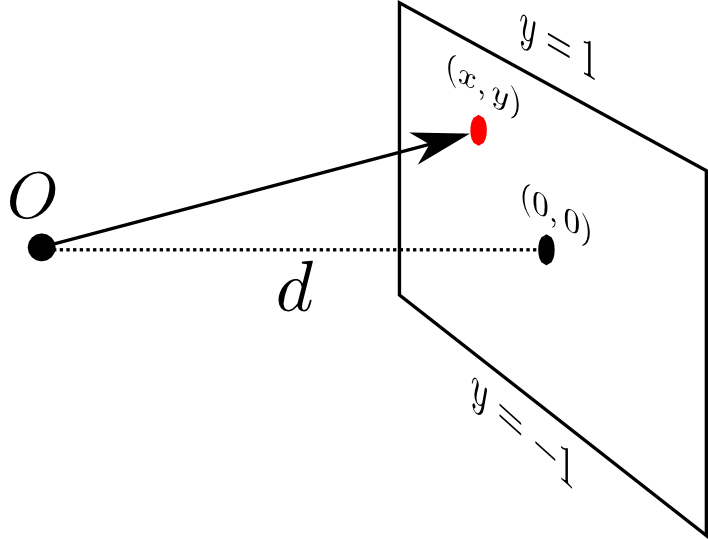
\includegraphics[width=0.4\textwidth]{fig1.png}
\end{center}
Assume our screen is positioned at distance $d$ from the origin. Let the center of the screen have pixel coordinates $(0, 0)$, the top and bottom correspond to pixel $y$ coordinate $1$ and $-1$ respectively. If we assume the camera is looking along the negative $z$ direction, the direction of a ray through pixel $(x,y)$ can be computed as $(x, y, -d)$. The parameter $d$ is related to the field of view angle $\alpha_y$:
$$\frac{1}{d} = \tan\left(\frac{\alpha_y}{2}\right).
$$

\paragraph{2. Cast the ray and look for intersections with objects in the scene.} Given the ray origin point $O$ (which corresponds to the camera position, i.e. $(0, 0, 0)$ in our case) and ray direction that we computed in the previous step, we can check for all primitives in the scene whether the ray intersects them, look for the closest one, and return the color of the pixel.

\begin{exercise}{1}{1.0}
The code base for this exercise is provided on the ShaderToy at \url{https://www.shadertoy.com/view/ldSGzW}. Examine the code. We would like to raycast the following scene:
\begin{center}
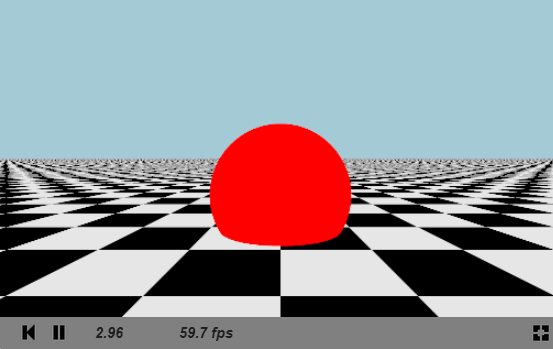
\includegraphics[width=0.7\textwidth]{raycasting.png}
\end{center}
The scene consists of a red sphere and a plane with a checkerboard pattern. The code base provides the specifications for both the plane and the sphere in the variables \texttt{plane}, \texttt{sphere}. The colors of the sky and sphere are provided in the \verb#sky_color# and \verb#sphere_color# variables. The function \verb#plane_color# takes a point on the plane and returns its color.

The methods for finding ray-object intersection are also provided: functions \verb#raycast_plane# and \verb#raycast_sphere# return the distance from ray origin to the intersection with the object, or \verb#INFINITY# if the ray does not hit the object. You need to introduce three changes to the code:
\begin{enumerate}
\item First implement the function \verb#raycast_scene#. The function should return the color of the object, hit first by the given ray.
\item Then fix the main function so that the resulting image would have a field of view of 60 degrees along the $y$ axis.
\item At this point you will see the scene rendered. However, it will have a lot of aliasing artifacts: the sphere has jagged edges and the checkerboard pattern turns into nonsense at a distance. Let us fix this using a simple 3x3 discrete box filter. That is, rather than using a single ray for pixel $(x,y)$, cast 9 rays, as if you would be rendering pixels $\{x-0.2, x, x+0.2\}\times\{y-0.2, y, y+0.2\}$, and average the results\footnote{You are free to try larger grids, however note that having long nested loops in shader code may lead to weird results on some graphics cards.}. 
\end{enumerate}
\end{exercise}

\end{document}
